\باب{سوالات}

\حصہء{ترچھی آمد}
%=================
\ابتدا{سوال}
دائیں دائری قطبی موج  نیم لامحدود پلیکسی گلاس  \عددی{(\sigma=0,\mu_R=1,\epsilon_R=3.45)} کی سطح پر بریوسٹر زاویے سے آمد ہے۔آمدی کثافت طاقت \عددی{\SI{100}{\watt\per\meter\squared}} ہے۔الف) پلیکسی گلاس کا بریوسٹر زاویہ حاصل کریں۔ ب) \عددی{\Gamma_{\parallel}} اور \عددی{\Gamma_{\perp}} حاصل کریں۔ پ) انعکاسی اور ترسیلی کثافت طاقت دریافت کریں۔ ت) انعکاسی اور ترسیلی امواج کی قطبیت بیان کریں۔ (آمدی دائری قطبی موج میں آدھی طاقت عمودی برقی اور آدھی طاقت متوازی برقی ہو گی۔)

جوابات:\عددی{61.7^{\circ}}، \عددی{\Gamma_{\parallel}=0}، \عددی{\Gamma_{\perp}=-0.549}، \عددی{\SI{15}{\watt\per\meter\squared}}، \عددی{\SI{85}{\watt\per\meter\squared}}، انعکاسی موج خطی قطبی جبکہ ترسیلی موج بیضوی قطبی ہے۔
\انتہا{سوال}
%=================
\ابتدا{سوال}
شکل \حوالہ{شکل_ترچھی_شیش_ریشہ} میں شیش ریشہ دکھایا گیا ہے۔اس شیش ریشے میں بائیں جانب سے شعاع \عددی{\theta} زاویے سے داخل ہوتی ہے۔یہ شعاع غلاف سے مکمل اندرونی انعکاس کرتے ہوئے شیش ریشے کے دوسرے سر تک پہنچتی ہے۔بیرونی خلاء کا انحرافی مستقل \عددی{n_0=1} لیتے ہوئے \عددی{\theta} کی وہ حد دریافت کریں جس کے اندر رہتے ہوئے  شیش ریشے میں مکمل اندرونی انعکاس پائی جائے گی۔\عددی{\sin \theta} کو شیش ریشے کی \اصطلاح{عددی شگاف}\فرہنگ{عددی شگاف}\حاشیہب{numerical aperture}\فرہنگ{numerical aperture} کہتے ہیں۔   
\begin{figure}
\centering
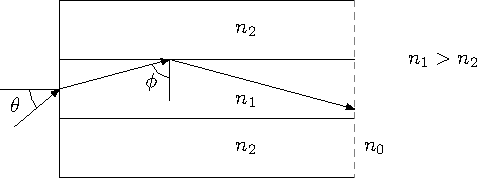
\includegraphics{figObliqueOpticalFiber}
\caption{شیش ریشہ۔}
\label{شکل_ترچھی_شیش_ریشہ}
\end{figure}

جواب:\عددی{\theta_{\text{بلندتر}}=\sin^{-1} \sqrt{n_1^2-n_2^2}}
\انتہا{سوال}
%=======================
\ابتدا{سوال}
شکل \حوالہ{شکل_ترچھی_شیش_ریشہ} میں \عددی{\theta} بریوسٹر زاویہ اور \عددی{\phi} زاویہ فاصل ہونے کی صورت میں \عددی{n_0} کو \عددی{n_1} اور \عددی{n_2} کی صورت میں بیان کریں۔

جواب:\عددی{n_0=\frac{n_1}{n_2}\sqrt{n_1^2-n_2^2}}
\انتہا{سوال}
%=====================
\ابتدا{سوال}
ایسا منشور جو  متوازی برقی موج کو بغیر گھٹائے گزرنے دے \اصطلاح{بریوسٹر منشور}\فرہنگ{منشور!بریوسٹر}\حاشیہب{Brewster prism}\فرہنگ{prism!Brewster} کہلاتا ہے۔ شکل \حوالہ{شکل_ترچھی_منشور} میں دکھائے منشور کو \عددی{n=1.45} کے شیشے سے بنایا گیا ہے۔اس شکل میں دکھائی گئی صورت حال کو دیکھتے ہوئے زاویہ \عددی{\alpha} حاصل کریں۔ (داخلی اور خارجی شعاع شیشے کے عمود کے ساتھ بریوسٹر زاویہ بناتے ہیں۔اس سے انعکاسی ضیاع کا خاتمہ حاصل کیا جاتا ہے۔)
\begin{figure}
\centering
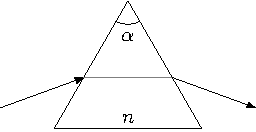
\includegraphics{figObliquePrismBrewster}
\caption{منشور}
\label{شکل_ترچھی_منشور}
\end{figure}

جواب:یہاں منشور کے اندر شعاع، منشور کے قاعدے کے متوازی ہے۔ \عددی{\alpha=69.2^{\circ}}
\انتہا{سوال}
%=====================
\ابتدا{سوال}
شکل \حوالہ{شکل_ترچھی_منشور} میں دکھائے گئے بریوسٹر منشور میں عمودی برقی موج کا کتنا فی صد گزر پائے گا۔

جواب:\عددی{\SI{76}{\percent}}
\انتہا{سوال}
%======================
\ابتدا{سوال}
شکل \حوالہ{شکل_ترچھی_منشور_سمت_تبدیل} میں شعاع کی سمت \عددی{90^{\circ}} تبدیل کرنے کی خاطر منشور استعمال کیا گیا ہے۔انعکاسی ضیاع سے چھٹکارے کی خاطر منشور کے بائیں اور بالائی سطحوں پر انعکاس مخلاف تہہ چڑھائی گئی ہے۔منشور کو خالی خلاء میں استعمال کرنے کی خاطر \عددی{n_1} کی کم سے کم قیمت دریافت کریں۔ 
\begin{figure}
\centering
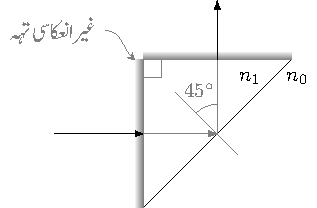
\includegraphics{figObliquePrismNintyDegreeReflection}
\caption{منشور سے شعاع کی سمت تبدیل کی جا سکتی ہے}
\label{شکل_ترچھی_منشور_سمت_تبدیل}
\end{figure}

جواب:\عددی{n_1>1.41}

\انتہا{سوال}
%=============================
\ابتدا{سوال}
دائری قطبی برقی موج دو عدد خطی قطبی امواج کے مجموعے سے بنی ہوئی ہے۔خطی قطبی امواج \عددی{E_x=5\cos(\omega t -\beta z)} اور \عددی{E_y=5\cos(\omega t -\beta z -90^{\circ})} ہیں۔ یہ دائری قطبی موج خطہ-1 \عددی{(\mu_{R1}=1, \epsilon_{R1}=1)} سے خطہ-2  \عددی{(\mu_{R2}=1, \epsilon_{R2}=3.5)} کے سرحد پر \عددیء{45^{\circ}} زاویے سے  پہنچتی ہے۔زاویہ سرحد کے عمود کے ساتھ ناپا جاتا ہے۔انعکاسی موج کی شرح رداس حاصل کریں۔

جواب:\عددی{2.38}
\انتہا{سوال}
%==================================
\ابتدا{سوال}
دائری قطبی برقی موج خطہ-1 \عددی{(\mu_{R1}=1, \epsilon_{R1}=1)} سے خطہ-2  \عددی{(\mu_{R2}=1, \epsilon_{R2}=4)} کے سرحد پر \عددی{\theta} زاویے سے  پہنچتی ہے۔زاویہ سرحد کے عمود کے ساتھ ناپا جاتا ہے۔ انعکاسی موج کی شرح رداس مندرجہ ذیل صورتوں میں حاصل کریں۔ الف) \عددی{\theta=30^{\circ}}،
 ب)\عددی{\theta=60^{\circ}}، پ) \عددی{\theta=63.43^{\circ}}

جواب:\عددی{1.35}، \عددی{10.9}، \عددی{7409}
\انتہا{سوال}
%=============================
\ابتدا{سوال}
دائیں بیضوی قطبی برقی موج از خود عمودی قطبی موج  \عددی{E_x=8\cos(\omega t -\beta z)} اور متوازی قطبی موج \عددی{E_y=6\cos(\omega t -\beta z -90^{\circ})}  کا مجموعہ ہے۔یہ دائیں بیضوی قطبی موج خطہ-1 \عددی{(\mu_{R1}=1, \epsilon_{R1}=1)} سے خطہ-2  \عددی{(\mu_{R2}=1, \epsilon_{R2}=3)} کے سرحد \عددی{z=0} پر \عددیء{30^{\circ}} زاویے سے  پہنچتی ہے۔زاویہ سرحد کے عمود کے ساتھ ناپا گیا ہے۔انعکاسی موج کی شرح رداس حاصل کریں۔

جواب:\عددی{2.68}
\انتہا{سوال}
%==================================

\ابتدا{سوال}
دائیں بیضوی قطبی برقی موج از خود عمودی قطبی موج  \عددی{E_x=8\cos(\omega t -\beta z)} اور متوازی قطبی موج \عددی{{E_y=6\cos(\omega t -\beta z -90^{\circ})}}  کا مجموعہ ہے۔یہ دائیں بیضوی قطبی موج خطہ-1 \عددی{(\mu_{R1}=1, \epsilon_{R1}=1)} سے خطہ-2  \عددی{(\mu_{R2}=1, \epsilon_{R2}=3)} کے سرحد \عددی{z=0} پر \عددیء{60^{\circ}} زاویے سے  پہنچتی ہے۔زاویہ سرحد کے عمود کے ساتھ ناپا گیا ہے۔انعکاسی موج کی شرح رداس حاصل کریں۔اس کی قطبیت بھی دریافت کریں۔

جواب:شرح رداس لامحدود ہے۔موج عمودی قطبی ہے۔
\انتہا{سوال}
%==================================
